%-- einleitung

\section{Konzept}

\subsection{Anforderungsanalyse}
Funktionale Anforderungen
Die Liste der Städte (Namen + Distanzen) sollen aus einer Datei (mit bestimmter Formatierung) auslesbar sein, damit diese Daten ohne Programmieraufwand verändert werden können.
Das System soll mit Genetischen Algorithmen das Travelling Salesman Problem umsetzen.
Das System soll Routen auf Grundlage derer Gesamtdistanz beurteilen und weiterverarbeiten.

Nichtfunktionale Anforderungen
Das System soll auf Windows 10 ausführbar sein.
Das System soll vollständig dokumentiert sein.
Das System soll leicht testbar sein.
Das System soll leicht bedienbar sein.
Das System soll als Executable ausführbar sein


\subsection{Systemmodellierung}

\begin{figure}[H]
\centering
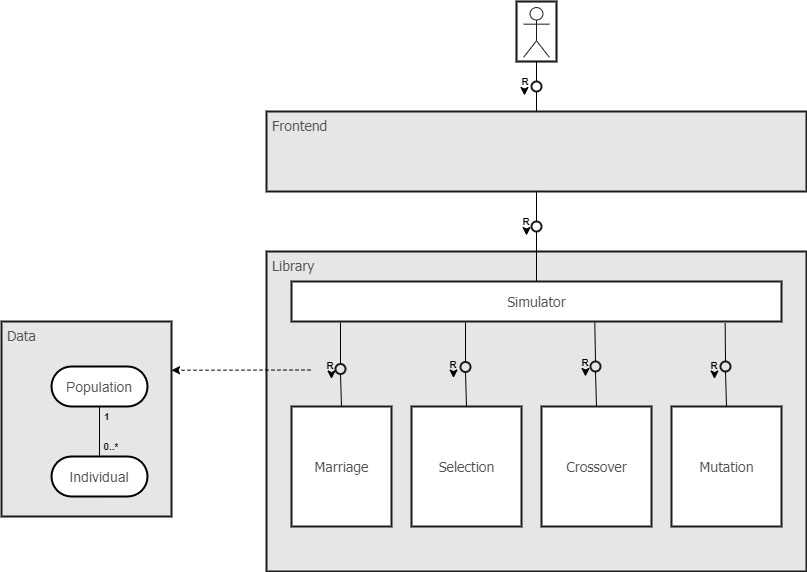
\includegraphics[width=1\textwidth]{img/Vortrag/Systemmodellierung.png}
\caption{Systemmodellierung}
\label{fig:systemmodellierung}
\end{figure}

%--